In this section, we apply our nonparametric model to a dataset of near-Earth astronomical objects (comets and asteroids).
We implemented the CRP-based sampler of the previous section in $\mathtt{R}$, with cluster parameters updated using the HMC sampler from the parametric case.
Inferences were based on $5,000$ samples from the MCMC sampler, after a burn-in period of $1,000$ samples.
%In all instances, we ran our MCMC sampling algorithm to produce $5000$ samples. We discarded the first $1000$ as burn-in samples,
%and made all inference using the remaining samples.

\subsection{Near Earth Objects dataset}
%We consider a dataset of orbits of near-earth objects (in particular,
%comets and asteroids).
The Near Earth Objects dataset was collected by the
Near Earth Object Program of the National Aeronautics and Space Administration\footnote{Downloaded from
$\mathtt{http://neo.jpl.nasa.gov/cgi-bin/neo\_elem}$}, and consists of $162$ observations. Each data point
lies on the Stiefel manifold $V_{3,2}$, and characterizes the orientation of a two-dimensional elliptical orbit in
%More precisely, the two directions give the latitude and longitude of perihelion of the two-dimensional orbit in
three-dimensional space.
The left subplot in Figure \ref{fig:neo_data} shows these data, with each $2$-frame represented as two orthonormal unit vectors.
The first component (representing the latitude of perihelion) is the set of cyan lines arranged as two horizontal cones.
The magenta lines (arranged as two vertical cones) form the second component, the longitude of perihelion.
%The bold lines (in blue and red) form a tightly clustered set of orientations of about $60$ orbits.
  \begin{figure}
  \centering
    \includegraphics[width=.4\textwidth]{figs/comets.pdf}
%    \includegraphics[width=.56\textwidth]{figs/comet_clstr.pdf}
  \centering
    \includegraphics[width=.3\textwidth]{figs/comets_adj.pdf}
\caption{The Near Earth Objects dataset (left), and the adjacency matrix inferred by the DP mixture model (right)}
  \label{fig:neo_data}
  \end{figure}
  \begin{figure}
  \centering
    \includegraphics[width=.35\textwidth]{figs/plot_nc.pdf}
  \centering
    \includegraphics[width=.42\textwidth]{figs/neo_3clstr.pdf}
\caption{Posterior over the number of clusters for the Near Earth Objects dataset (left), and location and scale parameters of an MCMC sample with
three clusters (right). The circles associated with each cluster correspond to $75\%$ predictive probability regions for the associated component.}
  \label{fig:post_nc}
  \end{figure}


We model this dataset as a DP mixture of matrix Langevin distributions. We set the DP concentration parameter $\alpha$
to $1$, and
for the DP base measure, %as in Section \ref{sec:Bays_inf},
placed independent probability measures on the matrices $G$ and $\bkappa$. % as in the parametric case (section \ref{sec:Bays_inf}). For the former
%(a point on the Stiefel manifold $V_{3,2}$)
For the former, we used a uniform prior (as in Section \ref{sec:Bays_inf}); %(a matrix Langevin distribution parametrized by an all-zero matrix).
%Recall that $\kappa$ is a square matrix with positive diagonal
%elements and zeros everywhere else.
however we found that an uninformative prior on $\bkappa$ resulted in high posterior probability for a single diffuse cluster
with no interesting structure.
% with
%small values of $\bkappa$.
To discourage this, we sought to penalize small values of $\kappa_i$. One way to do this is to
use a Gamma prior %on the diagonal elements of $\kappa$,
with a large shape parameter. Another is to use a hard constraint to bound the
$\kappa_i$'s away from small values. We took the latter approach, placing independent exponential priors restricted to $[5,\infty)$ on the
diagonal elements of $\bkappa$.

The right plot in Figure \ref{fig:neo_data} shows %the results of our nonparametric analysis.
%This subfigure shows
the adjacency matrix summarizing
the posterior distribution over clusterings. An off-diagonal element $(i,j)$ gives the number of times observations $i$ and $j$ were assigned to the
same cluster under the posterior. %, so that this term gives the posterior probability that these two elements belong to the same cluster.
We see a highly coupled set of observations (from around observation $20$ to $80$ keeping the ordering of the downloaded dataset). This cluster
corresponds to a tightly grouped set of observations, visible as a pair of bold lines in the left plot of Figure \ref{fig:neo_data}.

  \begin{figure}
  \centering
    \includegraphics[width=.48\textwidth]{figs/sph1_sc.pdf}
  \centering
    \includegraphics[width=.48\textwidth]{figs/sph2_sc.pdf}
\caption{Log predictive probabilities of first and second orthonormal components.}
  \label{fig:samplers_clst}
  \end{figure}
% \begin{figure}
% \centering
%   \includegraphics[width=.48\textwidth]{figs/comets_2_clstr.pdf}
% \centering
%   \includegraphics[width=.48\textwidth]{figs/comets_3_clstr.pdf}
%caption{Location and scale parameters of an MCMC sample with two (left) and three (right) clusters}
% \label{fig:samplers_clst}
% \end{figure}
To investigate the underlying structure more carefully, we plot in Figure \ref{fig:post_nc} the posterior distribution over the number of
clusters. % the observations are assigned to.
The figure shows this number is peaked at $4$, extending up to $9$. However, in most instances, most clusters
have a  small number of observations, with the posterior dominated by $2$ or $3$ large clusters.
%Figure \ref{fig:samplers_clst} shows the cluster of parameters from two samples,
%one with  two clusters, and one with three. The former is fairly typical of realizations with two clusters,
A typical two cluster realization is fairly intuitive, with
each cluster corresponding to one of the two pairs of cones at right angles, and these
clusters were identified quite consistently across all posterior samples.
Occasionally, one or both of these might be further split into two smaller clusters, resulting in $3$ or $4$
clusters. A different example of a three cluster structure is shown in the right subfigure (this instance corresponded to the last MCMC sample of our chain
that had three large clusters).
In addition to the two aforementioned clusters,
this assigns the bunched group observations mentioned earlier to their own cluster.
Parametric analysis of this dataset typically requires identifying this cluster and treating it as a single observation \citep{Sei2013440}, by contrast, our
nonparametric approach handles this much more naturally.

Finally, Figure \ref{fig:samplers_clst} show the log predictive-probabilities of observations given this dataset, with the left subplot giving the distribution of
the first component, and the right, the second. The peak of this distribution (the red spot to the right for the first plot, and the spot to the bottom left for the second),
correspond to the bunched set of observations mentioned earlier.
%\subsection{Vectorcardiogram dataset}  \label{sec:vcg_np}
%
%  \begin{figure}
%  \centering
%    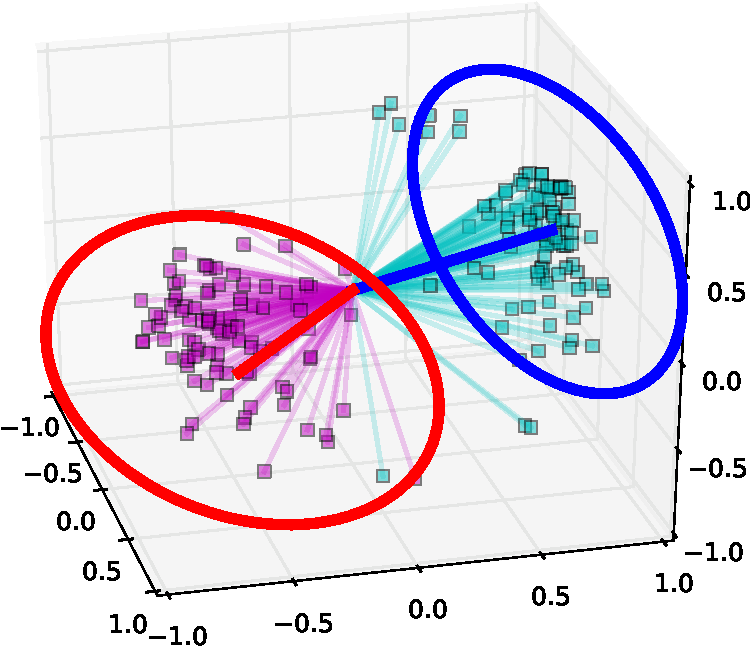
\includegraphics[width=.54\textwidth]{figs/vcg_post.pdf}
%  \centering
%    \includegraphics[width=.4\textwidth]{figs/plot_nc_vcg.pdf}
%\caption{Vector cardiogram dataset with inferred parameters (left), and the posterior over the number of clusters (right)}
%  \label{fig:samplers_comp}
%  \end{figure}
%The vectorcardiogram (VCG) is a loop traced by the \emph{cardiac vector} during a cycle of the heart beat. The two directions of orientation of this
%loop in
%three-dimensional space forms a point on the Stiefel manifold. The VCG dataset is a collection of $98$ such recordings,
%and is displaced in figure \ref{fig:samplers_comp}. Running our nonparametric analysis on this dataset reveals (as the data suggests) that
%there is no obvious clustering structure, with the data well modelled by a parametric Matrix Langevin distribution. For instance, the
%posterior distribution over the number of clusters is restricted mainly to values less than $2$ (with most probability assigned to $1$).
%In this instance, our nonparametric prior reduces to the simpler parametric distribution. An interesting future direction is to use such ideas to
%build and study nonparametric tests of whether or not the observed data belongs to some parametric family on the Stiefel manifold.

%%to data of comets from Marsden [1972], but did not consider Fisher distribution
%%on SO(3). See also Mardia [1975] for analysis of data of perihelion direction.
